% !TEX encoding = UTF-8 Unicode

\documentclass[12pt,oneside]{amsart}
\usepackage{cancel}
\usepackage{xspace}
\usepackage{graphicx}
\usepackage{multicol}
\usepackage{subfig}
\usepackage{amsmath}
\usepackage{amssymb}
\usepackage[a4paper,width=165mm,top=20mm,bottom=25mm,includeheadfoot]{geometry}
\usepackage{array}
\usepackage{verbatim}
\usepackage{caption}
\usepackage{natbib}
\usepackage{float}
\usepackage{pdflscape}
\usepackage{mathtools}
\usepackage[usenames,dvipsnames]{xcolor}
\usepackage{afterpage}
\usepackage{tikz}
\usepackage[bookmarks=true, unicode=true, pdftitle={Nexty Yellow Paper: a formal specification of Nexty, a zero transfer fee and instant transfer base on Ethereum blockchain}, pdfauthor={Thanh Dao / Ha Dang},pdfkeywords={Nexty, Ethereum, Yellow Paper, blockchain, virtual machine, cryptography, decentralised, singleton, transaction, generalised, zero transfer fee, instant transfer},pdfborder={0 0 0.5 [1 3]}]{hyperref}
%,pagebackref=true

\PassOptionsToPackage{hyphens}{url}\usepackage{hyperref}

\makeatletter
 \newcommand{\linkdest}[1]{\Hy@raisedlink{\hypertarget{#1}{}}}
\makeatother
\usepackage{seqsplit}

% For formatting
%\usepackage{underscore}
%\usepackage{lipsum} % to generate filler text for testing of document rendering
\usepackage[english]{babel}
\usepackage[autostyle]{csquotes}
\MakeOuterQuote{"}

\definecolor{pagecolor}{rgb}{1,0.98,0.9}

%Path relative to the main .tex file 
\graphicspath{ {./images/} }

\title{NEXTY: A CONSENSUS TO GET ZERO TRANSFER FEE AND INSTANT TRANSFER BLOCKCHAIN}
\author{
	Thanh Dao \& Ha Dang \\
	Co-founder/CTO @ Nexty Platform \\
	thanhdao@nexty.io / hadang@nexty.io
}
\date{} % delete this line to display the current date

%%% BEGIN DOCUMENT
\begin{document}

\pagecolor{pagecolor}
\begin{abstract}
This is the detail technical paper of \href{https://nexty.io}{Nexty Platform}, focusing on describing the operation of a consensus protocol called Proof of Foundation. Proof of Foundation was inspired by the Proof of Authority introduced by \cite{clique} with improvement from \href{https://nexty.io}{Nexty Platform} by introducing a new confirmation system named \textbf{DCCS} - \textbf{D}ual \textbf{C}ryptocurrency \textbf{C}onfirmation \textbf{S}ystem to achieve a absolutely decentralized system and bring a highly incentive system for blockchain maintainers.
\end{abstract}

\maketitle

\setlength{\columnsep}{20pt}
\begin{multicols}{2}
%\tableofcontents

\section{Introduction}\label{sec:introduction}
In addition to {\small NTY} coin-base, {\small DCCS} has the secondary token named {\small NTF}. {\small NTF} is used for authorizing an account to become the maintainer/sealer of the confirmation system described detail in section \ref{sec:authorize}, as well as to calculate reward for block sealer. {\small NTF} token has total supply of $10,000,000$ and will be distributed for the first $100,000,000,000$ NTY holders that joined in ``Smart Staking'' program described detail in the white paper of \cite{smart-taking}. In the other words, {\small NTF} will be rewarded to the pioneers having a clear vision and a strong believe in \href{https://nexty.io}{Nexty Platform} in the future. That's the reason why we call the new consensus protocol as \textit{``Proof of Foundation''}. The power of \href{https://nexty.io}{Nexty Platform}, however, is not belong to {\small NTF} holders because they could be voted down by Nexty community if community found that {\small NTF} holders did any bad behavior of cheating, malicious or hand-shaking to make the network become centralize chain as well as using out-of-date source code. As a result, {\small NTF} holders have the only role as block sealer for Nexty blockchain and governed  by {\small NTY} community via decentralize voting system on a smart contract.

\section{How to authorize an account to become a block sealer}\label{sec:authorize}
The system will set up a configuration parameter to determine the minimum value, $min-ntf$, that an account need to have to become block sealer. Nexty will build and develop a smart contract, which allow {\small NTF} token holder, having enough token, to grant another account called ``executing-account'' to become the block sealer by setting ``authorized-sealer'' state in the smart contract with the value equal to address of {\small NTF} holder. If an address already has an ``authorized-sealer'' value, it can not receive authorization from another NTF holder until the NTF holder has made the withdrawal it from ``authorized-sealer''. The ``authorized-sealer'' list will be determined at the check point block of each sealing round by reading state from the smart contract at that point of time. If in the current sealing round, any ``authorized-sealer'' does not perform at least one sealing activity, the ``authorized-sealer'' value will be withdrawn to its {\small NTF} holder by updating the state of the smart contract at the checkpoint block number of the next sealing round and of course that ``authorized-sealer'' will not be involved in the next sealing rounds until it will be authorized to become ``authorized-sealer'' again.

\section{Block sealing mechanism}\label{sec:sealing}
The {\small DCCS} block sealing mechanism will be implemented  as in following steps. Firstly, the sealers will be numbered from $1$ to $n$ (called ``sealing-id'') randomly at the beginning of each sealing round; in which, $n$ is the number of registered ``authorized-sealer'' and is determined by the state of the smart contract at the \textit{checkpoint block number} of the corresponding sealing round. To ensure the randomness of ``sealing-id'', the numbering is calculated by a hash,  $\boldsymbol{\xi_{\mathrm{k}}}$, as following formula when starting a new sealing round.

\begin{equation}
\xi_{\mathrm{k}} \equiv \texttt{\small KEC}(\mathbf{block}, \mathbf{\Lambda_{\mathrm{k}}})
\end{equation}

\begin{description}
\item[block] is the first block number, a.k.a  \textit{checkpoint block number} of the sealing round.
\item[$\Lambda_{\mathrm{k}}$] is the address that the {\small NTF} holder has set as ``authorized-sealer'' in the smart contract.
\item[\texttt{\small KEC}] is the \textbf{\small {SHA-3 Keccak-512}} hash function of any input.
\end{description}

After that, the ``sealing-id'' of each authorized-sealer will be taken by the position of \textit{sealing hash}, $\boldsymbol{\xi_k}$, in the array $(\xi_{\mathrm{1}}, \xi_{\mathrm{2}}, ..., \xi_{\mathrm{n}})$, ascending ordered by the \textit{sealing hash}.

To ensure performance of the system, the ``sealing-id'' of the all authorized sealers will be snapshot only once from the smart contract state at the \textit{checkpoint block number} of each sealing round and stored in the local database as well as in \textbf{lru cache} of each node.

\subsection{Scenario 1}\label{ch:scenario_1} If sealing node is not in recent sealers. The node will determine whether it's the in-turn sealer for the next block or not, according to the following formula:

\begin{equation}\label{eq:sigma}
\sigma_{\mathrm{k}} \equiv (\nu - \mathbf{block}) \ \ \ \mathbf{mod} \ \ \ \Pi
\end{equation}

\begin{description}
\item[$\nu$] is the current block number that is being sealed.
\item[block] is the first block number, a.k.a \textit{checkpoint block number}, of the current sealing round.
\item[$\Pi$] total number of authorized sealer reading from smart contract state at the \textit{checkpoint block} of the current sealing round.
\end{description}

If the remainder $\sigma_{\mathrm{k}}$ equal to ``sealing-id'' of the node, then that node has the right to seal block immediately. Otherwise, at each of the next block, sealing nodes have to wait a course of time, $\psi_{\mathrm{k}}$, which is calculated by the formula:

\begin{eqnarray}
\alpha = 001.387978000 \\
\beta = 000.002313279 \\
\gamma = 000.004626590 \\
\delta = 199.999400000
\end{eqnarray}

\begin{equation}\label{eq:psi}
\psi_{\mathrm{k}} \equiv \sum_{i=1}^{\zeta_\mathrm{k}} \mathbf{floor}(\frac{\alpha}{\beta*i+\gamma} + \delta)
\end{equation}

\subsection{Scenario 2}\label{ch:scenario_2} If sealing node is in recent sealers

In this scenario, sealers still can continue to seal block, but they have to wait a period of time longer than all other sealers, not in recent sealers. This is procedure to ensure that the system can still generate blocks, even when there is only one sealer, but the chain be suspended for a very long time. The waiting time ranges from $3$ - $30$ minutes, if there are $1,000$ - $10,000$ authorized sealers and only one or few active sealers.

Waiting time, $\psi_{\mathrm{k}}$,  is caculated by the following formula:

\begin{eqnarray}
\alpha = 001.387978000 \\
\beta = 000.002313279 \\
\gamma = 000.004626590 \\
\delta = 199.999400000
\end{eqnarray}

\begin{multline}\label{eq:psi_2}
\psi_{\mathrm{k}} \equiv \sum_{i=1}^{n} \mathbf{floor}(\frac{\alpha}{\beta*i+\gamma} + \delta) \\ 
+ \sum_{i=1}^{\zeta_\mathrm{k}} \mathbf{floor}(\frac{\alpha}{\beta*i+\gamma} + \delta)
\end{multline}

The coefficients of the above formula are assumed as following. The sealing node having ``sealing-id'' equal to $\sigma_{\mathrm{k}}$, calculated by formula $\eqref{eq:sigma}$, will have the priority to seal block before 400ms, the next sealing node will have the priority to seal block before 350ms, then 320ms,... till the final sealing node with approximately to 200ms. Its graph corresponds to the function $\texttt{\small y} = \frac{a} {(b * x + c)} + \texttt{\small d}$

To estimate values for the parameters, we use curve fitting method to find relatives coefficient in the website \href{https://mycurvefit.com/}{My Curve Fit} with the variance \footnote{R² is 1 minus the ratio of sum of the squares of the residuals divided by the sum of the squares of the differences between Y fit and the mean Y value} $\approx 1$.
\\
\\
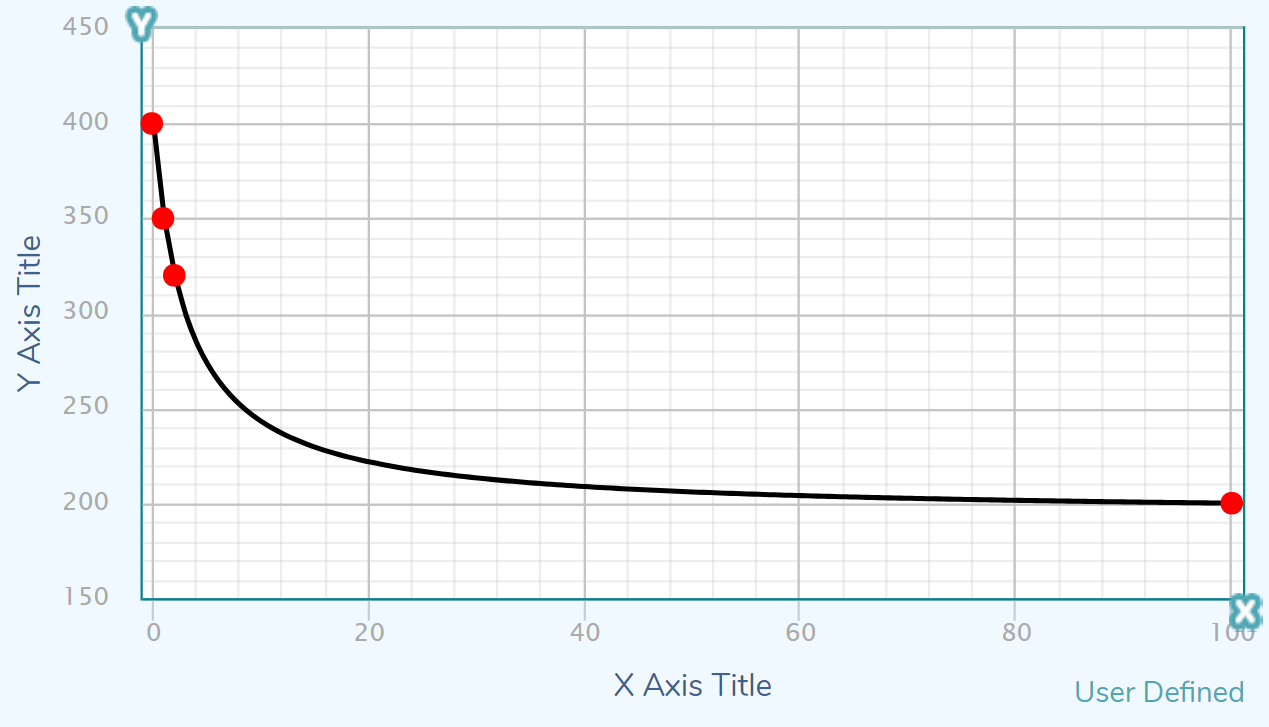
\includegraphics[width=0.48\textwidth, height=4cm]{curve-fit}
\\
A sealing round of all authorized sealer is called an epoch. Epoch will have various length, depends on the number of sealers in a chain of each sealing round.

A sealer who is worried about being withdrawn authorized sealer to {\small NTF} holder might not participate in sealing activity in a sealing round, but still occupies the right to seal block at some point earlier than his/her sealing turn; causes welter and racing for sealing block. By calculating the fixed waiting time for each sealer, using formula $\eqref{eq:psi}$ or $\eqref{eq:psi_2}$, consensus are able to keep track of sealer. Nexty blockchain will verify a block, sealed by an ``authorized-sealer'', by figuring out if the generating time of ``authorized-sealer''’s block is smaller than it's waiting time. 

\section{Block sealer reward calculation}

After each sealing round, reward value $\Re$ of each sealer will be calculated as the minimum value of the total reward divided by the active sealers according to the proportion of {\small NTF} they have on the total {\small NTF} of the sealers who participated in the seal.
  
\begin{eqnarray}
\theta = \frac{\Omega}{N} \\
\phi = \frac{\Upsilon_{NTF}}{\Xi_{NTF}}
\end{eqnarray}

\begin{equation}\label{eq:re}
\Re \equiv \min(\theta, \phi)
\end{equation}

\begin{description}
\item[$\Omega$] total reward
\item[N] total number of active sealer of the current sealing round
\item[$\Upsilon_{NTF}$] amount of NTF token that the owner of active sealer is holding
\item[$\Xi_{NTF}$] total amount of NTF token that all active sealer are holding
\end{description}

According to formula $\eqref{eq:re}$, people who own {\small NTF} in a natural way will divide his/her {\small NTF} into many wallets in order to equip multiple sealers, instead of building only one sealer and spend too much  {\small NTF} on it. This ensures the Nexty chain will have sufficiently large number of nodes to make Nexty chain become highly decentralization, stability and robust.

Total reward $\Omega$ is the amount of {\small NTF} was produced after each sealing round, calculated as \textit{[reward generated in one block]} * \textit{[number of blocks generated in that sealing round]}.

The number of rewards generated for a block is equal to the number of rewards per year divided by $\mathbf{15,768,000}$, the expected number of block within one year (initial configuration of block time is 2 seconds).
 
The amount of rewards in a year is calculated in the following proportions:

\begin{center}
  \begin{tabular}{@{} cc @{}}
    \hline
    Year &  \% of circulating supply \\ 
    \hline
    1 & 10 \\ 
    2 & 5 \\ 
    3 & 2 \\ 
    4 & 1 \\ 
    5 & 1 \\     
    ... & ... \\ 
    ... & ... \\ 
    ... & ... \\ 
    n &  1 \\
    \hline
  \end{tabular}
\end{center}

\section{Anti-SPAM}\label{sec:spam}

Since Nexty's transaction fee is zero, if there is no proper anti-spam protection, it can easily be attacked by sending multiple transactions simultaneously, causing system blockage.

We have the following anti-spam methods:

The general rule is that the system will charge the first transaction with a fee of \textit{0.2 per account}, which will be added to the reward value of the sealing round. From subsequent transactions, the system will not charge transaction fees, but requires those accounts to run a continuous wallet application with the number of blocks equal to \textit{[0.0015 * gas-used]}, after that, they will be able to send next transactions.

Mobile wallet app is a light client version, as known as a block verifier (based on light client protocol standard) which has the ability to save transactions of the it's own account and contiguous accounts in \textit{Merkle Tree} and block headers. The responsibility of a light client is to verify all transactional information related to it, as well as validate the blocks generated afterward. There should be a comparison if the blockchain is interfered with more than 15 blocks backwards, then notify to the owner of the wallet that the system might be manipulated. In some case, community must be accessed to see if any errors occurred, and vote down on the ``authorized-sealers'' that caused the malicious data. Under this rule, a spam action that spends more than 56.7 times the amount of resources on the chain to confirm such a transaction. This results in a loss in resources for spammers and therefore, ruins their intention of spamming.

Users still have the option of creating a charged transaction in case they do not want to maintain block verifier.

For \textbf{{\small {dApp}}}, it can provide its own system of nodes to withstand the user's gas and then there may or may not be a charge on the user's gas depending on the development needs of the \textbf{{\small {dApp}}}.

\bibliographystyle{plainnat}
\bibliography{Biblio}

\end{multicols}
\end{document}